\documentclass[a4paper]{article}
\usepackage[english]{babel}
%	\usepackage{simplemargins}

%	\usepackage[square]{natbib}
\usepackage{amsmath}
\usepackage{amsfonts}
\usepackage{amssymb}
\usepackage{bbold}
\usepackage{graphicx}
\usepackage{blindtext}
\usepackage{hyperref}
\usepackage{amsthm}
\usepackage{float}
\newtheorem{theorem}{Theorem}
\newtheorem{lemma}{Lemma}
\usepackage{algorithm}
%	\usepackage{algorithmic}
\usepackage{algpseudocode}
%	\usepackage{algorithm2e}
\usepackage{booktabs}
\usepackage[export]{adjustbox}
\setcounter{MaxMatrixCols}{20}

\begin{document}
\pagenumbering{arabic}

\Large
\begin{center}
\textbf{Monte Carlo Simulation of the Ising Model}\\

\hspace{10pt}

% Author name and affiliation
\large
% BSc. Julio A. Medina$^1$ \\
Julio A. Medina \\
\hspace{10pt}
\small
Universidad de San Carlos de Guatemala\\
School of Physical Sciences and Mathematics\\
Master's Degree in Physics\\
\href{mailto:julioantonio.medina@gmail.com}{julioantonio.medina@gmail.com}\\
\end{center}

\hspace{10pt}

\begin{abstract}
In statistical mechanics, the Ising model describes the short-range interactions between the magnetic dipole moments of molecular spins in a theoretical model of a ferromagnetic material. The spins are arranged on an $n$-dimensional lattice and take discrete values. In this work, the Ising model is simulated using a Monte Carlo method in order to analyze its behavior and determine whether phase transitions, specifically continuous transitions, occur. Continuous phase transitions and finite-lattice-size effects were observed. These finite-size effects decrease as the lattice size is increased.
\end{abstract}

\normalsize
\section{Introduction}
The Ising model is the archetypal model for describing the behavior of ferromagnetic materials and the phase transitions that can occur in such systems, particularly the paramagnetic--ferromagnetic transition. This behavior can be observed by taking a piece of iron that has previously been magnetized by a sufficiently strong magnetic field, thereby producing a temporary magnet, and bringing it near a heat source. Its magnetic properties rapidly disappear as its temperature increases.

\subsection{Phase Transitions}
Phase transitions and critical phenomena are associated with a wide variety of physical systems, including simple fluids and fluid mixtures, magnetic materials, ferromagnets, superfluids, superconductors, and others. Van der Waals's doctoral thesis (1873) introduced the first successful theory explaining the continuity between the liquid and gaseous states of matter. The transition to ferromagnetism was also explained in the early twentieth century by a phenomenological theory proposed by Pierre Curie and developed by Weiss, which is closely related to van der Waals theory. These are known as classical theories of phase transitions and are still used to describe some qualitative aspects of many systems.\\

These classical theories underwent more rigorous analysis during the 1960s. Several thermodynamic quantities, such as specific heat, compressibility, and magnetic susceptibility, exhibit peculiar behavior in the so-called critical region, with asymptotic divergences characterized by a set of critical exponents. It was quickly recognized that the critical behavior of equivalent thermodynamic quantities exhibits a universal characterization that can be described by well-defined critical exponents.\\

\subsubsection{Landau Phenomenology}
Landau theory for continuous phase transitions is based on expanding the free energy in terms of invariants of the order parameter. The free energy is therefore assumed to be an analytic function, even in the neighborhood of a critical point. In many cases, it is relatively straightforward to identify a suitable set of order parameters associated with a phase transition. The order parameter is not always a scalar; it may even be a tensor in complex systems. In general, $\psi=0$ in the phase with greater symmetry, which usually occurs at high temperatures in the disordered phase, whereas $\psi\neq 0$ in the less symmetric and more ordered phase.\\

Examples of order parameters include:
\begin{itemize}
\item The liquid--gas transition, for which $\psi$ is given by $v_G-v_L$ or by $\rho_L-\rho_G$, where $v$ is the specific volume and $\rho$ is the particle density.
\item The paramagnetic--ferromagnetic transition, for which the order parameter $\psi$ may be the magnetization vector. In a uniaxial system such as the Ising model, it becomes a scalar in the absence of an applied field.
\item The antiferromagnetic transition, for which the order parameter $\psi$ may be associated with the sublattice magnetization.
\end{itemize}
The list is not exhaustive. For a pure fluid, the order parameter is a scalar and the expansion can be written as
\begin{equation}
g(T,p;\psi)=g_0(T,p)+g_1(T,p)\psi+g_2(T,p)\psi^2+g_3(T,p)\psi^3+g_4(T,p)\psi^4+\cdots,
\end{equation}
where the coefficients $g_n$ are functions of the thermodynamic fields $T$ and $p$. To obtain a simple critical point, it is sufficient for $g_4$ to be positive, ensuring the existence of a minimum with respect to $\psi$; higher-order terms are therefore omitted from the Landau expansion. Because there is some freedom in the choice of $\psi$, it is always possible to eliminate the cubic term from the expansion (see \cite{Salinas}). Thus, without loss of generality, the expansion can be written as
\begin{equation}
g(T,p;\psi)=A_0(T,p)+A_1(T,p)\psi+A_2(T,p)\psi^2+\psi^4.
\end{equation}
For a stable minimum, the coefficients $A_1$ and $A_2$ must vanish at the critical point. It is important to note, however, that the existence of such an expansion cannot be taken for granted; the exact solution of the two-dimensional Ising model is a well-known counterexample.\\

For a uniaxial ferromagnet, the Landau expansion is simpler because of symmetry, and the Helmholtz free energy can be written as
\begin{equation}
f(T,m)=f_0(T)+A(T)m^2+B(T)m^4+\cdots.
\end{equation}
This gives
\begin{equation}
g(T,H,m)=f_0(T)-Hm+A(T)m^2+B(T)m^4+\cdots.
\end{equation}
At the critical point, $H=0$ and $A(T)=0$. In the neighborhood of the critical point, one may write
\begin{equation}
A(T)=a(T-T_c),
\end{equation}
with $a>0$, $B(T)=b>0$, and $f_0(T)\approx f_0(T_c)$. Therefore,
\begin{equation}
g(T,H,m)=f_0(T_c)-Hm+a(T-T_c)m^2+bm^4.
\end{equation}

\subsection{The Ising Model}
Most experiments performed near critical points indicate that critical exponents take universal values that differ substantially from those predicted by classical theories, such as the example presented in the discussion of Landau phenomenology. It is now understood that the values of the critical exponents depend on only a few ingredients:
\begin{itemize}
\item The dimensionality of the physical system.
\item The dimensionality of the order parameter. For uniaxial ferromagnets, the order parameter is a scalar.
\item The range of the microscopic interactions.
\end{itemize}
Because of the universal behavior of critical exponents, it is sufficient to analyze simple but nontrivial systems such as the Ising model. The Ising model represents the ferromagnetic interactions among the molecules of a material as a discrete model. A discrete value is assigned to the relative orientation of each magnetic dipole moment, or spin. The value $+1$ is assigned to an orientation parallel to the $y$ axis of the lattice formed by the discretized molecular positions, as shown in Figure~1, whereas $-1$ is assigned to the antiparallel orientation.

\begin{figure}[H]
\begin{center}
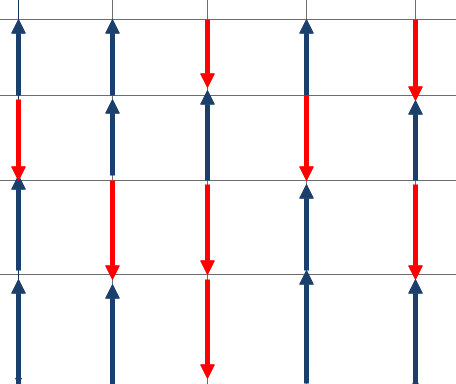
\includegraphics[scale=0.4]{LatticeIsing.png}
\end{center}
\caption{Spin lattice}
\end{figure}

The analysis considers interactions between neighboring spins $\sigma_i$, where $\sigma_i=\pm1$ represents the spin at position $(x,y)$ on the lattice. The interaction strength between neighboring spins is governed by a constant $J$, so the Hamiltonian of the system can be written as
\begin{equation}
\label{H1}
\mathcal{H}=-J\sum_{\langle ij\rangle}\sigma_i\sigma_j-H\sum_{i=1}^{N}\sigma_i.
\end{equation}
Here, $H$ is an external magnetic field applied to the region occupied by the molecular lattice, $N$ is the total number of molecules on the lattice, and the energy scale $J$ may be interpreted as a quantum-mechanical parameter associated with the microscopic interaction. In the first sum, $\langle ij\rangle$ denotes a sum over nearest-neighbor interactions. For example, the neighbors of the position $(x,y)$ are $(x,y+1)$, $(x,y-1)$, $(x-1,y)$, and $(x+1,y)$. These neighbors are shown in blue in Figure~2, whereas the site $(x,y)$ is shown in red. The first term in Equation~\ref{H1} represents the interaction energy that favors an ordered ferromagnetic state. The second term represents the interaction between the applied magnetic field $H$ and the spins of the system; this interaction is purely paramagnetic.

\begin{figure}[H]
\begin{center}
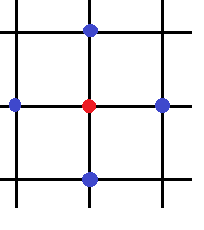
\includegraphics[scale=0.4]{Neighbor.png}
\end{center}
\caption{Nearest neighbors}
\end{figure}

For $H=0$, Equation~\ref{H1} becomes
\begin{equation}
\label{H2}
\mathcal{H}=-J\sum_{\langle ij\rangle}\sigma_i\sigma_j.
\end{equation}
To solve the Ising problem, the canonical partition function must be found:
\begin{equation}\label{partition}
Z(T,H,N)=\sum_{\{\sigma_i\}}\exp(-\beta\mathcal{H}),
\end{equation}
where $\beta=1/(K_B T)$, $K_B$ is the Boltzmann constant, and $T$ is the temperature in kelvin. From this partition function, the free energy per site is
\begin{equation}
g=g(T,H)=\lim_{N\to\infty}\left[-\frac{1}{\beta N}\ln Z_N\right].
\end{equation}
In one dimension, an expression for this free energy can be obtained relatively easily, for example through the transfer-matrix method, which may also be used in higher dimensions. However, the one-dimensional solution is misleading in the context of phase transitions, as shown by Ising (1925), because its analyticity in $T$ and $H$ precludes spontaneous magnetization and any finite-temperature phase transition.\\

Several approximation techniques have been developed to solve the Ising model in two and three dimensions. Some are relatively simple and useful, producing qualitatively reasonable phase diagrams. As mentioned above, phase transitions are associated with nonanalytic behavior of the free energy in the thermodynamic limit. Consequently, caution is required when using truncations or perturbative expansions near the critical point.\\

Lars Onsager (see \cite{Onsanger,Pathria}) found an exact analytical solution for the Ising model on a square lattice with nearest-neighbor interactions in the absence of an external field, $H=0$, as described by Equation~\ref{H2}. As $T\to T_c$, the specific heat diverges according to the asymptotic logarithmic form
\begin{equation}
c_{H=0}\sim \ln|T-T_c|,
\end{equation}
with the well-defined critical temperature
\begin{equation}\label{Tc}
T_c=\frac{2J}{K_B\ln(1+\sqrt{2})}.
\end{equation}
A brief presentation of the exact one-dimensional solution is given below. Approximation methods and a solution on the Bethe lattice can be found in Baxter (see \cite{Baxter}).

\subsection{Exact Solution of the One-Dimensional Ising Model}
In one dimension, the Hamiltonian in Equation~\ref{H1} becomes
\begin{equation}
\mathcal{H}=-J\sum_{i=1}^{N}\sigma_i\sigma_{i+1}-H\sum_{i=1}^{N}\sigma_i.
\end{equation}
The partition function is
\begin{equation}
Z_N=\sum_{\{\sigma_i\}}\exp\left[K\sum_{i=1}^{N}\sigma_i\sigma_{i+1}+\frac{L}{2}\sum_{i=1}^{N}(\sigma_i+\sigma_{i+1})\right],
\end{equation}
where $K=\beta J$ and $L=\beta H$. The second term has been rewritten in a more symmetric form. For convenience, periodic boundary conditions are imposed, that is, $\sigma_{N+1}=\sigma_1$. The partition function may be written as
\begin{equation}\label{canonical_partition_fucntion}
Z_N=\sum_{\sigma_1,\sigma_2,\ldots,\sigma_N}\prod_{i=1}^{N}T(\sigma_i,\sigma_{i+1}),
\end{equation}
where
\begin{equation}
T(\sigma_i,\sigma_{i+1})=\exp\left[K\sigma_i\sigma_{i+1}+\frac{L}{2}(\sigma_i+\sigma_{i+1})\right].
\end{equation}
The last expression can be represented as a $2\times2$ matrix whose indices are the spin variables $\sigma_i=\pm1$ and $\sigma_{i+1}=\pm1$. This defines the transfer matrix:
\begin{equation}
\mathbf{T}=
\begin{pmatrix}
T(+,+) & T(+,-)\\
T(-,+) & T(-,-)
\end{pmatrix}
=
\begin{pmatrix}
\exp(K+L) & \exp(-K)\\
\exp(-K) & \exp(K-L)
\end{pmatrix}.
\end{equation}
Using matrix notation (see \cite{Salinas,Pathria}), the canonical partition function in Equation~\ref{canonical_partition_fucntion} can be expressed as the trace of the $N$th power of the transfer matrix:
\begin{equation}
Z_N=\operatorname{Tr}(\mathbf{T}^N).
\end{equation}
Because the transfer matrix is symmetric, it can be diagonalized by a unitary transformation:
\begin{equation*}
\mathbf{U}\mathbf{T}\mathbf{U}^{-1}=\mathbf{D},
\end{equation*}
where $\mathbf{U}^{-1}=\mathbf{U}^{\dagger}$ and $\mathbf{D}$ is diagonal. The canonical partition function can therefore be expressed in terms of the eigenvalues of the transfer matrix:
\begin{equation}
Z_N=\operatorname{Tr}\left[(\mathbf{U}^{-1}\mathbf{D}\mathbf{U})^N\right]=\operatorname{Tr}(\mathbf{D}^N)=\lambda_1^N+\lambda_2^N.
\end{equation}
The eigenvalues, obtained from the characteristic equation $\det(\mathbf{T}-\lambda\mathbf{I})=0$, are
\begin{equation}\label{eigen_values}
\lambda_{1,2}=e^K\cosh L\pm\left(e^{2K}\sinh^2L+e^{-2K}\right)^{1/2}.
\end{equation}
These eigenvalues are always positive and $\lambda_1>\lambda_2$, except at the trivial point $T=H=0$. In the absence of an external field, $L=0$, one obtains
\begin{equation}
\lambda_1=2\cosh K\geq \lambda_2=2\sinh K,
\end{equation}
and the state becomes degenerate, $\lambda_1=\lambda_2$, in the limit $K\to\infty$, which is equivalent to $T\to0$. To obtain the free energy, it is convenient to write the partition function as
\begin{equation}
Z_N=\lambda_1^N\left[1+\left(\frac{\lambda_2}{\lambda_1}\right)^N\right].
\end{equation}
Since $\lambda_1>\lambda_2$, the thermodynamic limit is easily evaluated:
\begin{equation}
g(T,H)=\lim_{N\to\infty}\left[-\frac{1}{\beta N}\ln Z_N\right]= -\frac{1}{\beta}\ln\lambda_1.
\end{equation}
Using Equation~\ref{eigen_values}, one obtains
\begin{equation}
g(T,H)=-\frac{1}{\beta}\ln\left\{e^{\beta J}\cosh(\beta H)+\left[e^{2\beta J}\sinh^2(\beta H)+e^{-2\beta J}\right]^{1/2}\right\},
\end{equation}
which is analytic in $T$ and $H$, and from which all thermodynamic properties of the one-dimensional system can be derived. The average magnetization per site is
\begin{equation}
m(T,H)=-\left(\frac{\partial g}{\partial H}\right)_T=\frac{\sinh(\beta H)}{\left[\sinh^2(\beta H)+e^{-4\beta J}\right]^{1/2}}.
\end{equation}

\section{Methodology}
\subsection{Monte Carlo Method}
\subsubsection{Master Equation}
The master equation (see \cite{Salinas}) is introduced to describe the time evolution of Markovian stochastic processes. Let $P(y,t)$ be the probability of finding a system in microscopic state $y$ at time $t$. Differentiating this probability gives
\begin{equation}
\frac{\partial}{\partial t}P(y,t)=T_0-T_f,
\end{equation}
where the rate at which probability flows into state $y$ is
\begin{equation}
T_0=\sum_{y'}P(y',t)w(y'\rightarrow y),
\end{equation}
and $w(y'\rightarrow y)$ may be interpreted as the probability per unit time that the system moves from state $y'$ to state $y$. Analogously, the rate at which probability flows out of state $y$ is
\begin{equation}
T_f=P(y,t)\sum_{y'}w(y\rightarrow y').
\end{equation}
The master equation is therefore
\begin{equation}\label{masterEq}
\frac{\partial}{\partial t}P(y,t)=\sum_{y'}\left[P(y',t)w(y'\rightarrow y)-P(y,t)w(y\rightarrow y')\right].
\end{equation}
For a stationary state, $P(y,t)$ has no explicit time dependence, so equilibrium requires
\begin{equation}
\frac{\partial}{\partial t}P(y,t)=0.
\end{equation}
This leads to the equilibrium condition known as the principle of detailed balance:
\begin{equation}\label{equi}
P(y',t)w(y'\rightarrow y)=P(y,t)w(y\rightarrow y').
\end{equation}

\subsubsection{Monte Carlo Method}
The study of equilibrium systems in statistical mechanics is concerned with calculating averages of the form
\begin{equation}\label{MCavg}
\langle A\rangle=\frac{\displaystyle\sum_C A(C)\exp(-\beta\mathcal{H})}{\displaystyle\sum_C\exp(-\beta\mathcal{H})},
\end{equation}
where the sum includes all possible microscopic configurations of the system associated with the Hamiltonian $\mathcal{H}$. For a two-dimensional Ising model with an $n\times n$ lattice, the total number of sites is $N=n^2$, so the sum in Equation~\ref{MCavg} extends over $2^N=2^{n^2}$ configurations. Because the number of configurations grows as $2^{n^2}$, direct numerical evaluation is impractical. The solution is to average over a much smaller number of representative equilibrium configurations:
\begin{equation}\label{MCavg2}
\langle A\rangle\approx\frac{1}{M}\sum_{i=1}^{M}A_i.
\end{equation}
It is important to determine the conditions under which this arithmetic average over $M$ representative configurations approaches the expected value of $A$, as well as how the number $M$ should be chosen.\\

In the Monte Carlo method, a sequence of statistically generated configurations is selected through a Markov chain. Some initial configurations may be far from equilibrium, but as the process evolves, many configurations representative of equilibrium are generated and used in the average in Equation~\ref{MCavg2}.\\

As discussed above, if $w(y\rightarrow y')$ is identified as the transition probability per unit time from state $y$ to state $y'$, then the master equation in Equation~\ref{masterEq} and the detailed-balance condition in Equation~\ref{equi} apply.\\

At equilibrium, after a sufficiently long sequence has been generated, the probabilities should approach the Gibbs distribution:
\begin{equation}
P_0(y)=\frac{1}{Z}\exp[-\beta\mathcal{H}(y)],
\end{equation}
where $Z$ is the canonical partition function defined in Equation~\ref{partition}. From Equation~\ref{equi},
\begin{equation}
P_0(y)w(y\rightarrow y')=P_0(y')w(y'\rightarrow y).
\end{equation}
Transition probabilities are chosen to satisfy
\begin{equation}\label{probTans1}
\frac{w(y\rightarrow y')}{w(y'\rightarrow y)}=\exp(-\beta\Delta\mathcal{H}),
\end{equation}
where $\Delta\mathcal{H}=\mathcal{H}(y')-\mathcal{H}(y)$ is the energy difference between configurations $y$ and $y'$.\\

Two commonly used transition rules in Monte Carlo simulations are Glauber dynamics and the Metropolis prescription. The Metropolis prescription is used in this simulation:
\begin{equation}
w(y\rightarrow y')=
\begin{cases}
\dfrac{1}{\tau}\exp(-\beta\Delta\mathcal{H}), & \Delta\mathcal{H}>0,\\
\dfrac{1}{\tau}, & \Delta\mathcal{H}\leq0,
\end{cases}
\end{equation}
where the time scale $\tau$ is interpreted as a Monte Carlo step.

\subsubsection{Monte Carlo Method for the Ising Model}
The steps of the Monte Carlo method and the flowchart used to generate the Markov chain are presented below:
\begin{enumerate}
\item Choose an initial spin configuration on the lattice.
\item Select a site at random and calculate the energy change associated with flipping that spin, including its nearest-neighbor interactions and the external field.
\item Check the sign of $\Delta E$.
\item If $\Delta E\leq0$, flip the spin at the selected site, that is, set $\sigma_i\leftarrow-\sigma_i$.
\item If $\Delta E>0$ but $\exp(-\beta\Delta E)>p_t$, where $p_t$ is a random number between $0$ and $1$, flip the spin. Otherwise, reject the change and begin the next cycle.
\end{enumerate}
These steps implement a Monte Carlo simulation using the Metropolis prescription.

\begin{figure}[H]
\begin{center}
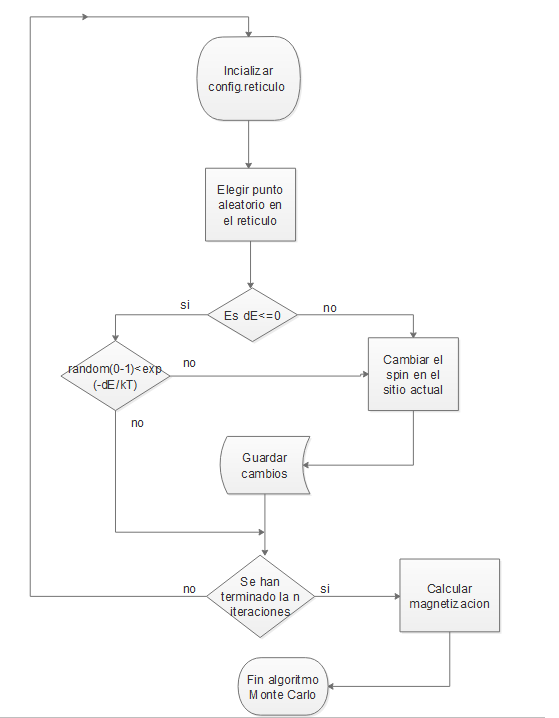
\includegraphics[scale=0.5]{FluxDiagram.png}
\end{center}
\caption{Flowchart}
\end{figure}

\subsection{Computation Times}
To characterize the computation time of the implementation of the Monte Carlo method with the Metropolis prescription, several simulations were performed to analyze how execution time changes as another parameter is varied.

\subsubsection{Lattice Size}
To analyze computation time as a function of lattice size, simulations were performed for lattice dimensions $N\in[10,500]$ in increments of $10$. The following figure shows how computation time increases with $N$. Each lattice contains $N\times N$ sites, and the number of Monte Carlo iterations was held fixed at $n=10000$.

\begin{figure}[H]
\begin{center}
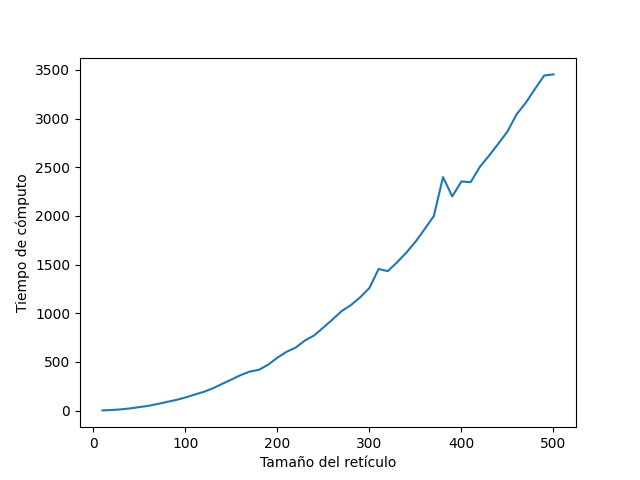
\includegraphics[scale=0.64]{time_vrs_lattice_size.png}
\end{center}
\caption{Computation time (s) versus $N$}
\end{figure}

\subsubsection{Temperature}
To analyze computation time as a function of temperature, a simulation was performed using a fixed lattice size $N=50$ while varying the temperature over $T\in[1,100]$. The number of Monte Carlo iterations was again fixed at $n=10000$. All simulations use theoretical-physics units in which $K_B=1$.

\begin{figure}[H]
\begin{center}
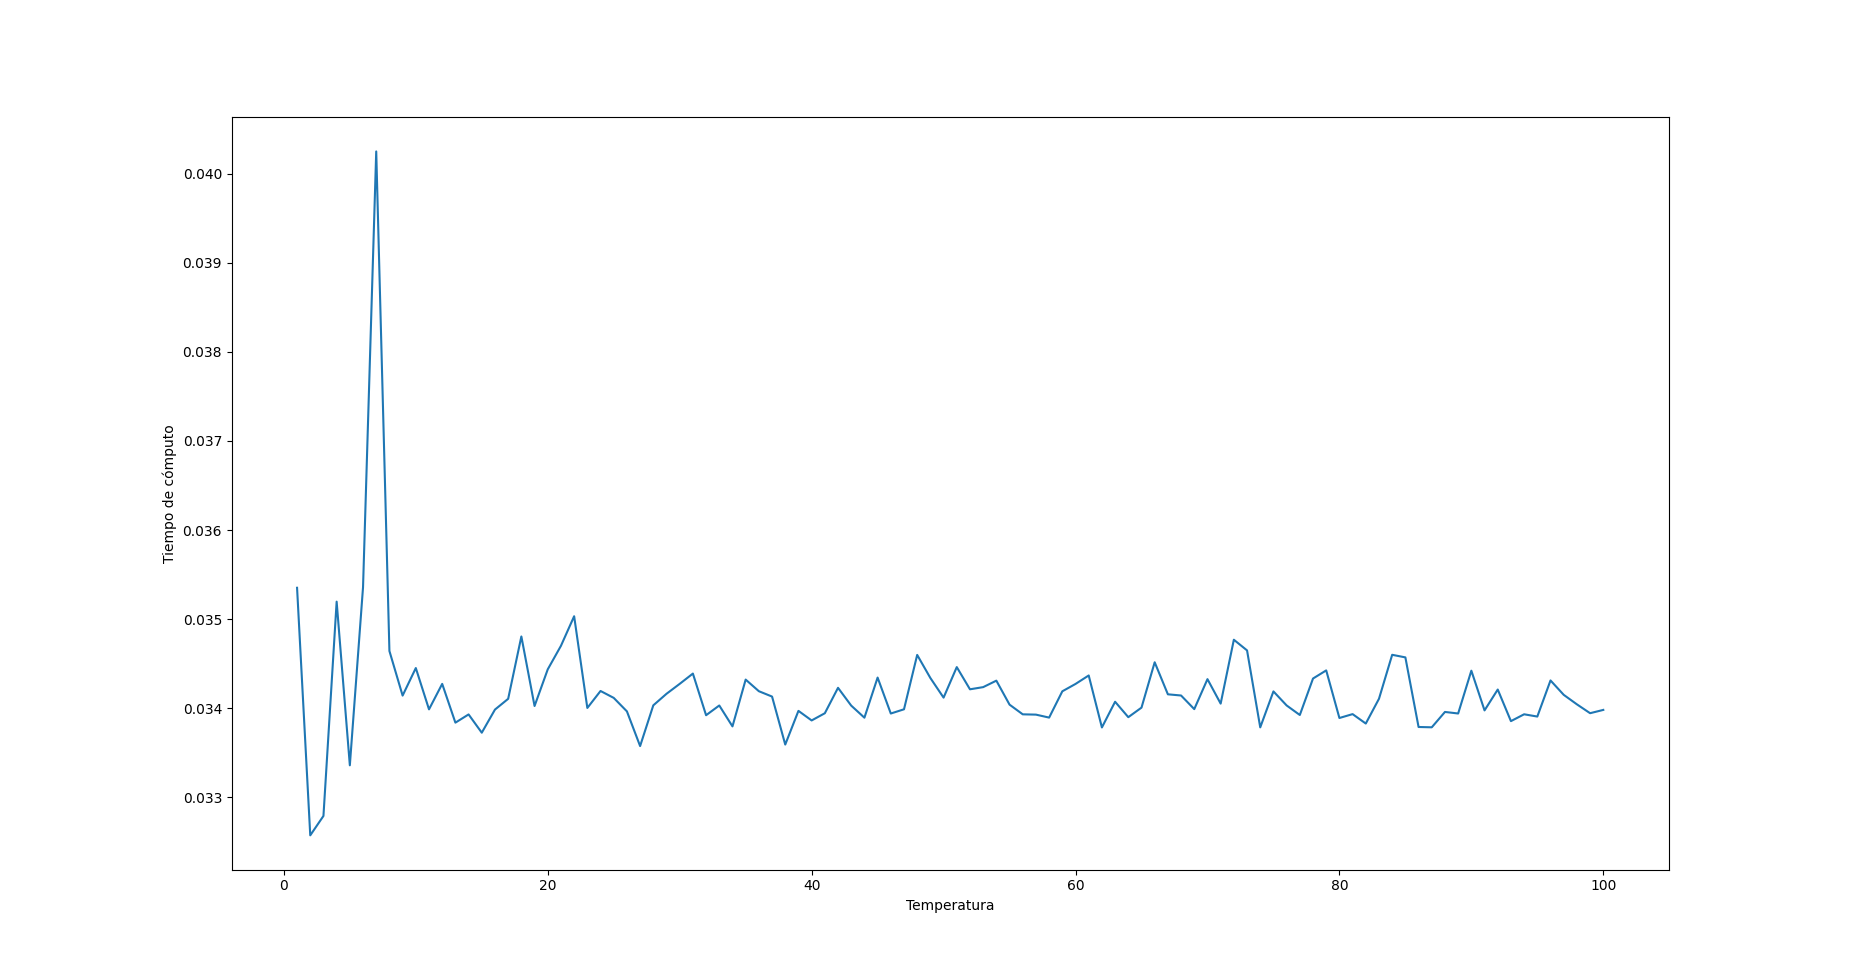
\includegraphics[scale=0.3]{time_vrs_T.png}
\end{center}
\caption{Computation time (s) versus temperature}
\end{figure}

For fixed $n$ (the number of iterations) and $N$ (the lattice dimension), the computation time remains approximately constant as the temperature changes. This is consistent with the implementation of the Monte Carlo algorithm for the Ising model. During this simulation, the average magnetization per site was also recorded as the temperature varied. A phase transition can be observed: the simulation begins with a magnetized material, which becomes completely demagnetized after a critical temperature is exceeded, corresponding to a ferromagnetic--paramagnetic transition.

\begin{figure}[H]
\begin{center}
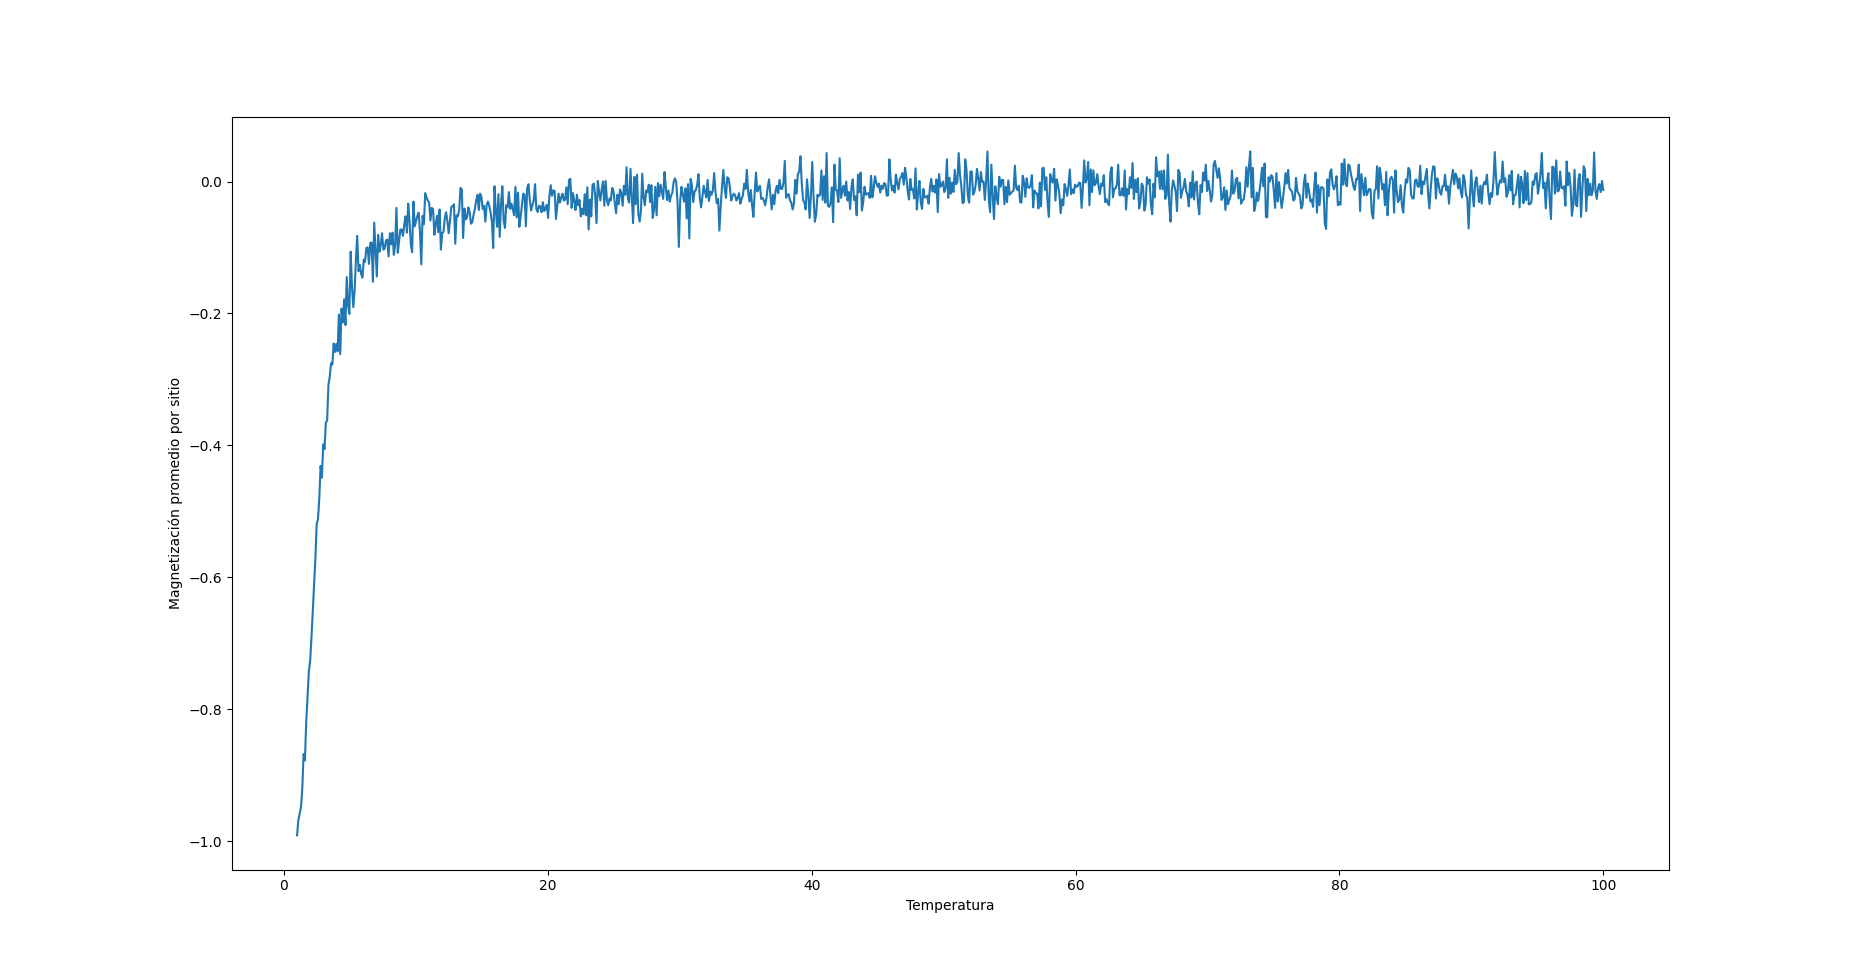
\includegraphics[scale=0.3]{M_vrs_T.png}
\end{center}
\caption{Magnetization versus temperature}
\end{figure}

\subsubsection{Number of Monte Carlo Iterations}
Another parameter of interest for evaluating computation time is the number of Monte Carlo iterations. In this case, $n\in[100,10000]$ was varied while the lattice size and temperature were fixed at $N=50$ and $T=5$, respectively. The computation time exhibits approximately linear growth, as shown in the following graph.

\begin{figure}[H]
\begin{center}
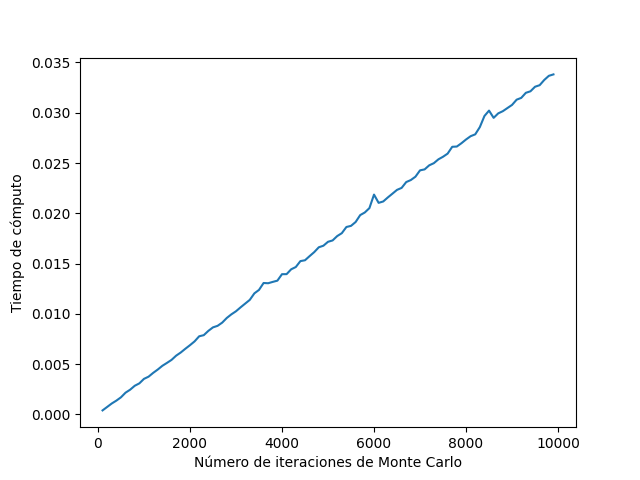
\includegraphics[scale=0.6]{time_vrs_MC_iterations.png}
\end{center}
\caption{Computation time (s) versus number of iterations}
\end{figure}

\section{Results}
The average magnetization can be used to evaluate the behavior of the Monte Carlo algorithm. Of particular interest is how the parameter $J$, which describes the interaction between spins, and the parameter $H$, which represents the strength of the external magnetic field in the Hamiltonian in Equation~\ref{H1}, affect the numerical simulation. The influence of the ratio $J/H$ on the overall behavior is also considered.\\

For $H=0$, the Hamiltonian reduces to Equation~\ref{H2}, and the only interactions are those between neighboring spins. A simulation was performed with $J=1$, lattice dimension $N=50$, and therefore $N\times N=2500$ lattice sites. The temperature was varied over $T\in[0.1,10]$, and $n=10000$ Monte Carlo iterations were performed. The chosen initial state had all spins set to $\sigma_i=-1$, so the ferromagnetic material was initially fully magnetized.

\begin{figure}[H]
\begin{center}
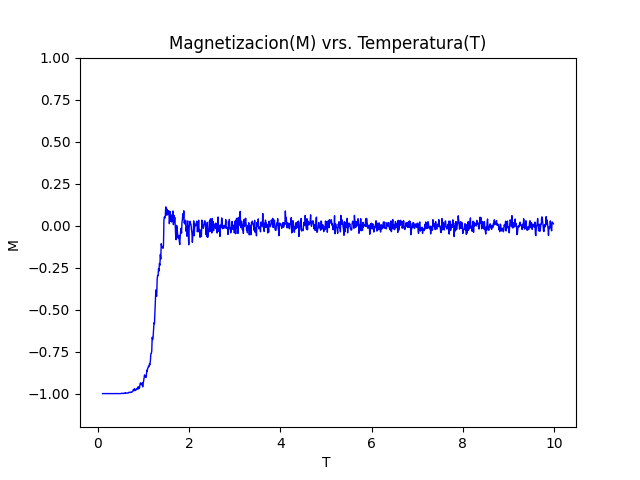
\includegraphics[scale=0.6]{PlotMvT_sim1.png}
\end{center}
\caption{Magnetization versus temperature}
\end{figure}

A phase transition can be clearly observed beyond a certain critical temperature. Once equilibrium is reached in the disordered phase, only small fluctuations remain around a magnetization of $M=0$. For $J=1$ and $K_B=1$, the exact critical temperature from Equation~\ref{Tc} is
\begin{equation}
T_c=\frac{2}{\ln(1+\sqrt{2})}\approx2.2692.
\end{equation}
In the following figure, this temperature is identified by a vertical red line.

\begin{figure}[H]
\begin{center}
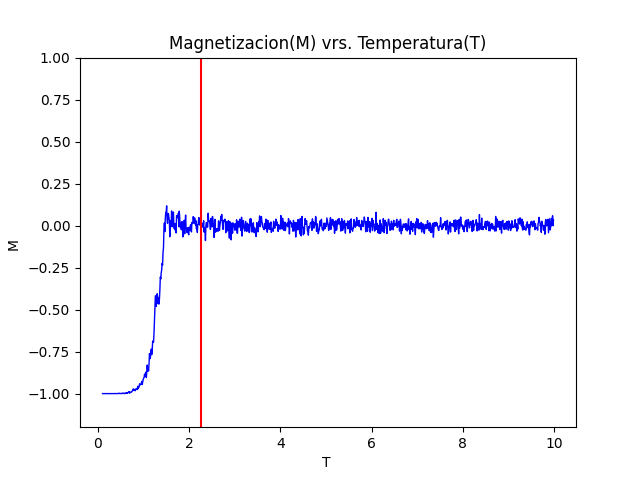
\includegraphics[scale=0.6]{PlotMvT_sim1_v02.png}
\end{center}
\caption{Magnetization versus temperature}
\end{figure}

Finite-lattice-size effects are visible. To investigate their influence on the numerical estimate of the critical point, another simulation was performed under the same conditions but with $N=500$, corresponding to a lattice of $N\times N=250000$ sites.

\begin{figure}[H]
\begin{center}
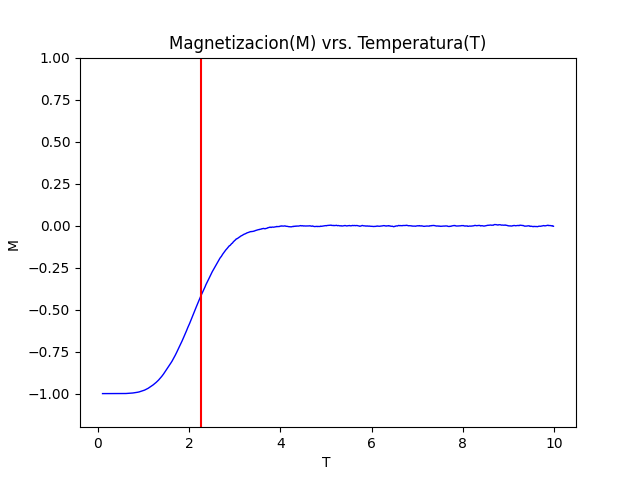
\includegraphics[scale=0.6]{PlotMvT_sim1_v03.png}
\end{center}
\caption{Magnetization versus temperature}
\end{figure}

Increasing the lattice size produces a better approximation to the critical point, suggesting that finite-size effects can be reduced by using larger lattices. Another important effect of increasing the lattice size is that the transition appears smoother, which is consistent with a continuous, or second-order, phase transition.\\

To confirm that the critical temperature can be estimated from the Monte Carlo simulation, a simulation was run with $J=0.5$. In theoretical units with $K_B=1$, Equation~\ref{Tc} gives $T_c\approx1.1346$.

\begin{figure}[H]
\begin{center}
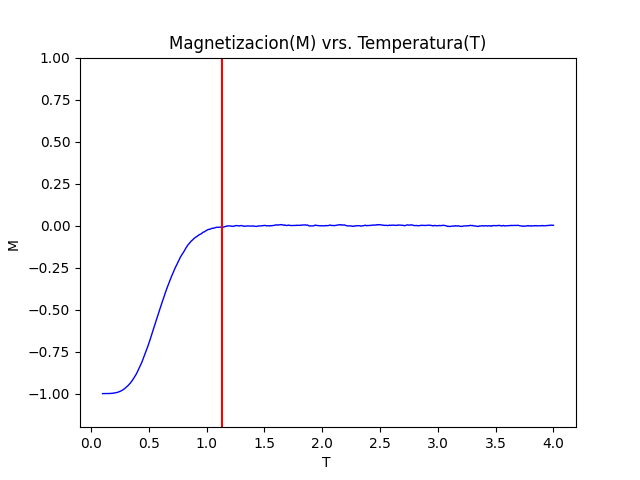
\includegraphics[scale=0.6]{PlotMvT_sim1_v04.png}
\end{center}
\caption{Magnetization versus temperature}
\end{figure}

For this case, $T\in[0,4]$. Changing the value of $J$ reduces the temperature at which the material becomes completely disordered and demagnetized, in agreement with the theoretical value of $T_c$, which is marked in red.\\

Under the same conditions as in the first case, $H=0$, $N\times N=2500$, and $n=10000$, but with all initial spins set to $\sigma_i=+1$, the following result is obtained:

\begin{figure}[H]
\begin{center}

\includegraphics[scale=0.6]{PlotMvT_sim2.png}
\end{center}
\caption{Magnetization versus temperature}
\end{figure}

The expected behavior is observed: the simulation begins with a magnetized ferromagnetic material and transitions to a state without net magnetic order.\\

For $J/H=1$, beginning from an initial state in which all spins are $\sigma_i=+1$, the following result is obtained:

\begin{figure}[H]
\begin{center}
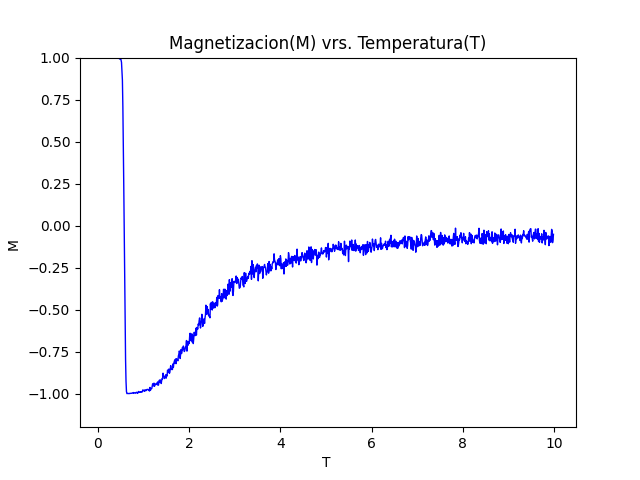
\includegraphics[scale=0.6]{PlotMvT_sim3.png}
\end{center}
\caption{Magnetization versus temperature}
\end{figure}

The influence of the external magnetic field $H$ is clearly visible. The system tends to align with the field and subsequently becomes increasingly disordered as the temperature rises. Animations of these processes are available in the \texttt{GitHub} repository at \url{https://github.com/Julio-Medina/Ising_Model/tree/main}.\\

For $J/H=1/10$, with $T\in[0.1,300]$ and the same remaining conditions as in the first case, the following result is obtained:

\begin{figure}[H]
\begin{center}
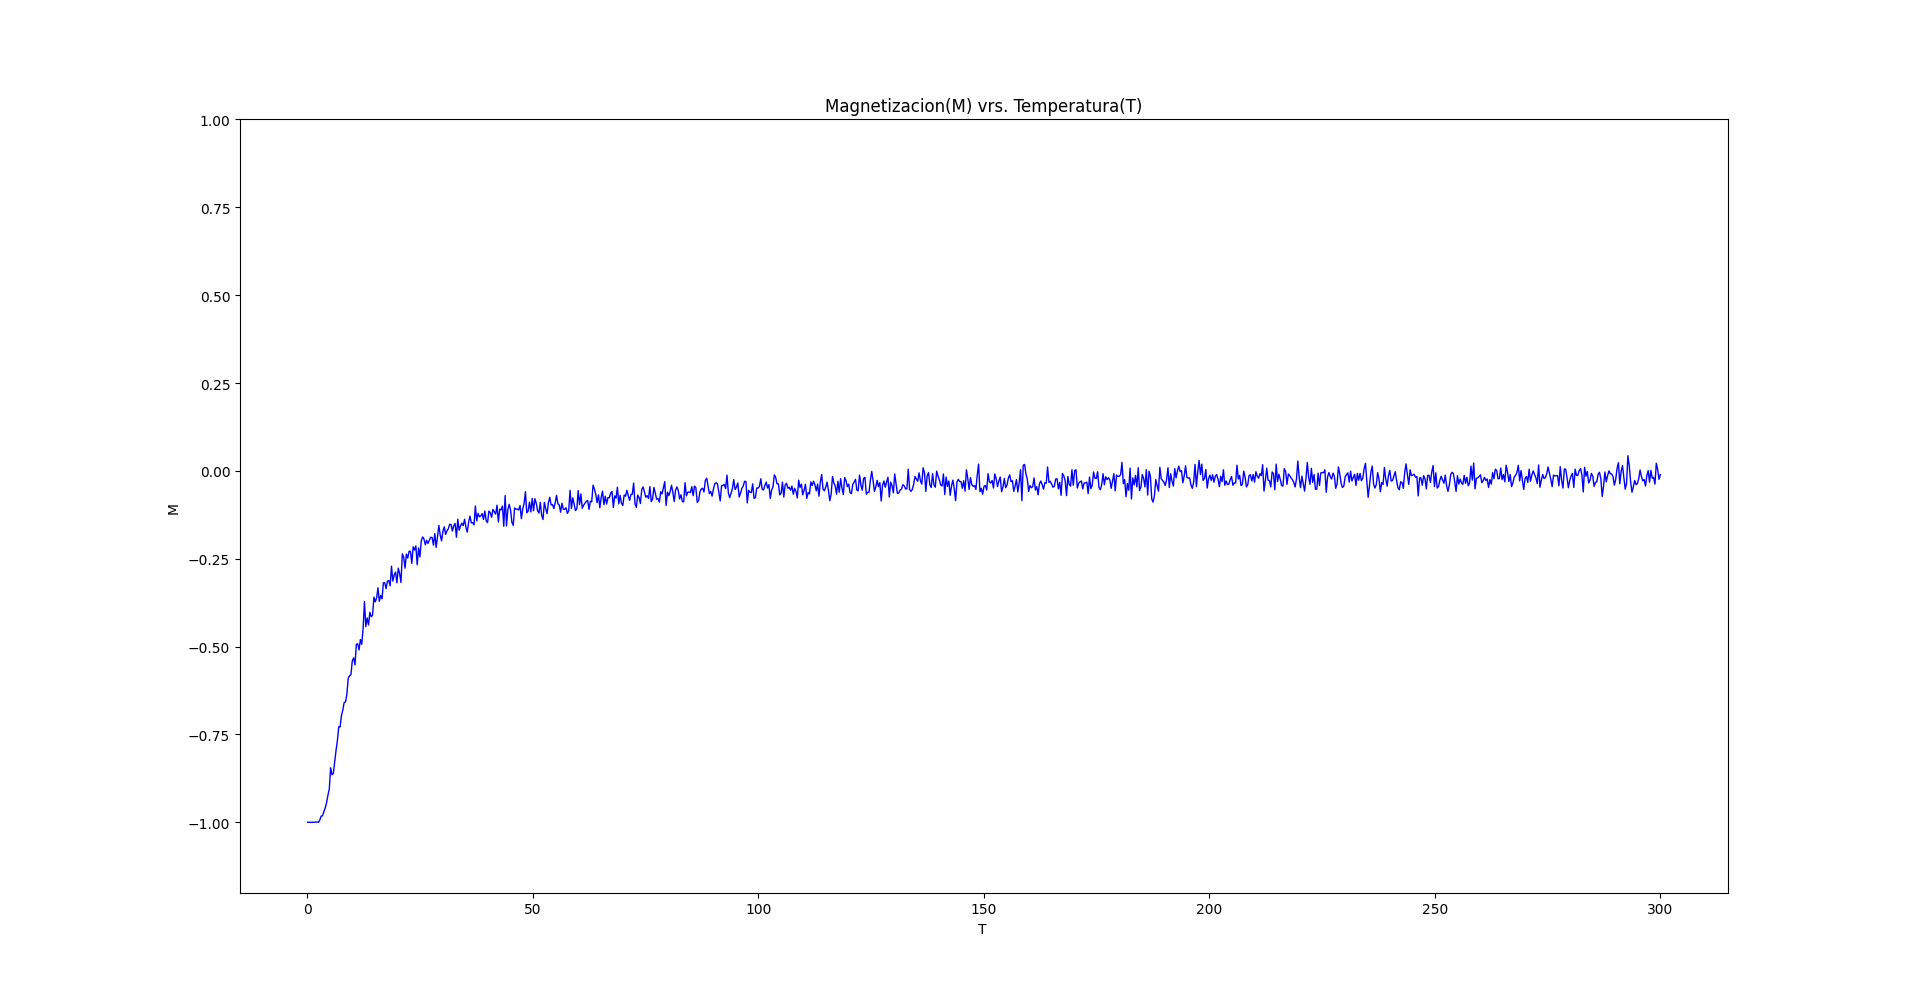
\includegraphics[scale=0.3]{PlotMvT_sim12.png}
\end{center}
\caption{Magnetization versus temperature}
\end{figure}

This case also shows the effect of a nonzero external field whose magnitude exceeds the spin--spin interaction scale. Higher temperatures are required to substantially disorder the system when the field is parallel to the initial magnetization. Strictly speaking, for $H\neq0$ the sharp zero-field critical point is replaced by a smooth crossover rather than a true thermodynamic phase transition.\\

For larger values of $J/H$, stronger spin--spin interactions preserve magnetic order to higher temperatures. The following simulation shows the case $J/H=2$:

\begin{figure}[H]
\begin{center}
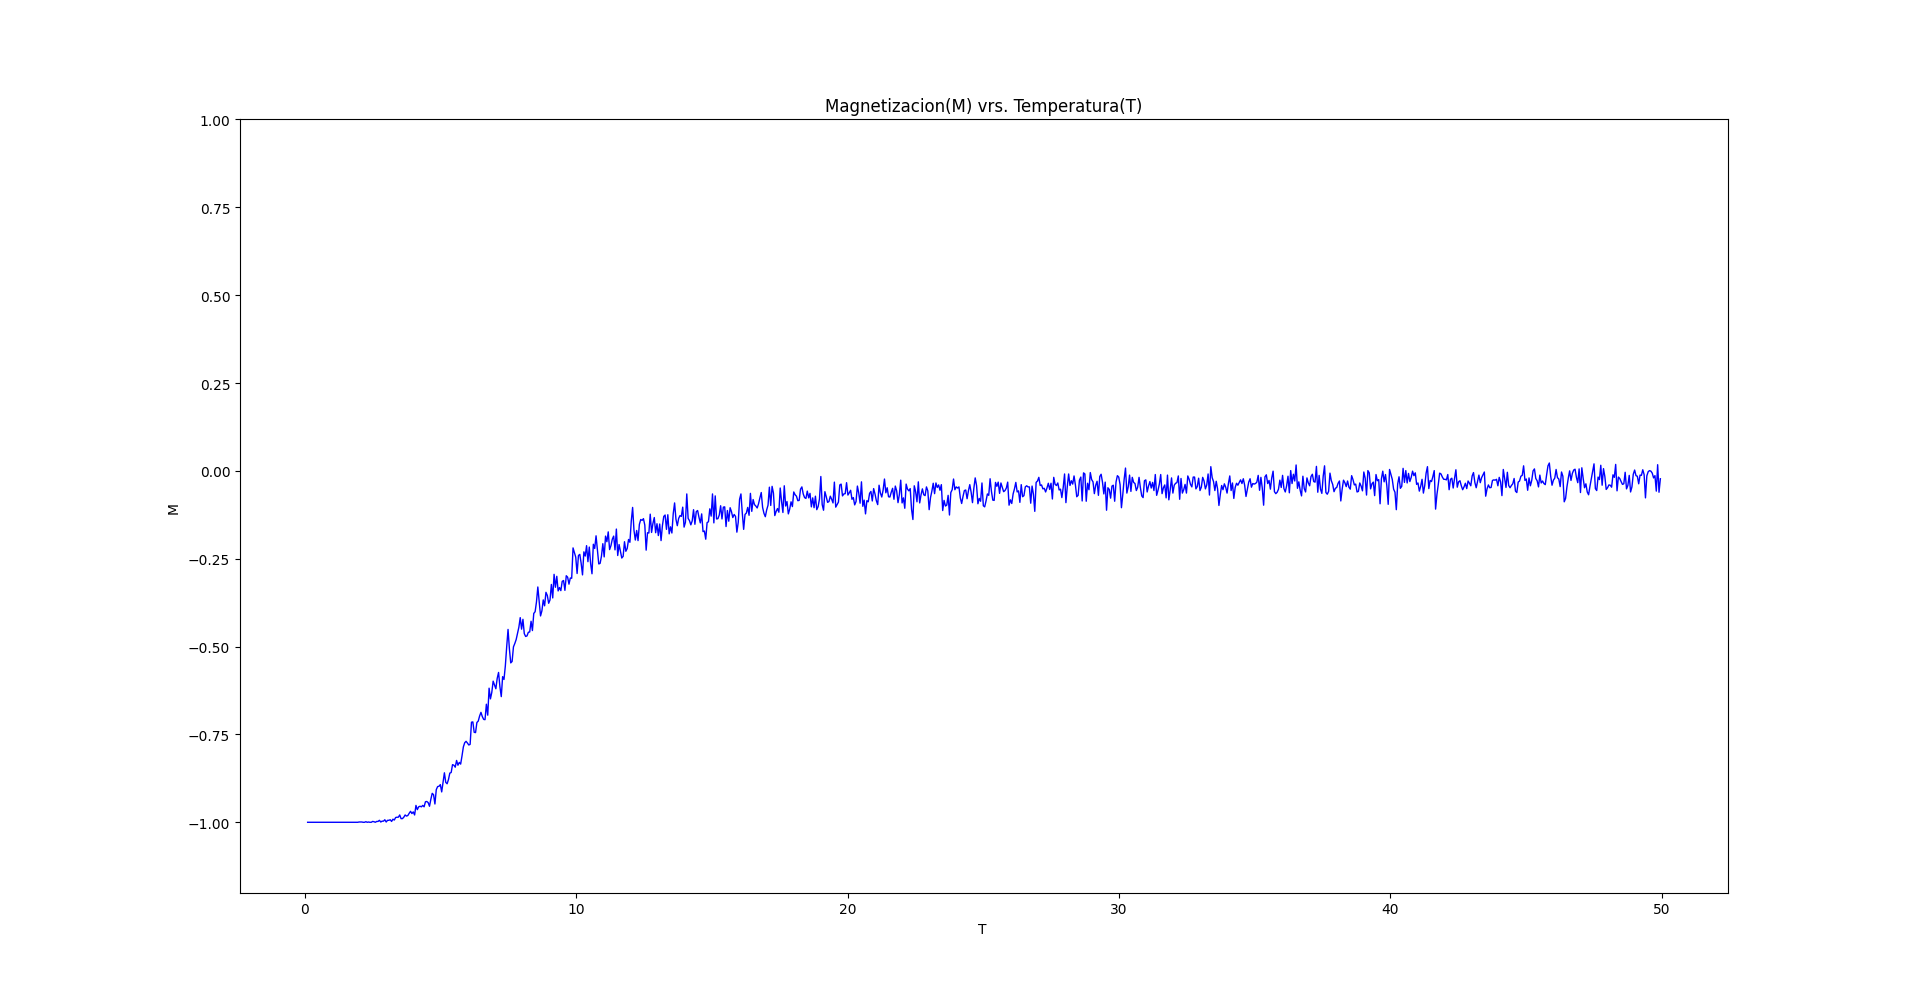
\includegraphics[scale=0.3]{PlotMvT_sim13.png}
\end{center}
\caption{Magnetization versus temperature}
\end{figure}

In this case, interactions between lattice spins are stronger, so significant changes in magnetization begin at higher temperatures. This is consistent with the expected behavior of the system.

\section{Conclusions}
The Monte Carlo method, implemented through the Metropolis prescription, provides a useful approach for approximating the behavior of the Ising model. In general, the simulations display the loss of magnetic order as temperature increases. For the zero-field two-dimensional model, the material loses its spontaneous magnetization above the critical temperature and approaches a disordered state, consistently with Onsager's exact result \cite{Onsanger}.\\

Finite-lattice-size effects can be reduced by using a sufficiently large lattice and an adequate number of Monte Carlo iterations. In general, the number of attempted spin updates must scale appropriately with the total number of lattice sites in order to obtain representative results for the two-dimensional Ising model.\\

The Monte Carlo simulations produced behavior broadly consistent with the analytical solution of the two-dimensional Ising model. The numerical behavior depends on the Hamiltonian parameters $H$ and $J$ in Equation~\ref{H1}. At zero field, the critical temperature scales with $J$ according to Equation~\ref{Tc}; when $H\neq0$, the field biases the magnetization and smooths the temperature-dependent response.

\begin{thebibliography}{99}
% The bibliography is ordered alphabetically by the surname of the author
% or principal author. Each entry is formatted according to whether it is
% a book, article, thesis, web resource, or another type of source.

\bibitem{Baxter} R. J. Baxter. \textit{Exactly Solved Models in Statistical Mechanics}. Academic Press, first edition.

\bibitem{Salinas} Silvio R. A. Salinas. \textit{Introduction to Statistical Physics}. Springer, first edition.

\bibitem{Onsanger} Lars Onsager. \textit{Crystal Statistics. I. A Two-Dimensional Model with an Order-Disorder Transition}. Physical Review 65, 117 (1944). \url{https://doi.org/10.1103/PhysRev.65.117}

\bibitem{Pathria} R. K. Pathria. \textit{Statistical Mechanics}. Elsevier, third edition.

\end{thebibliography}
\end{document}
